\chapter{Fourier Series}
\section{波的Time Domain与空域}
谈频率的时候,时间就不再是一个变量。
\begin{enumerate}
	\item 空间固定,使用frequency表示一秒内经过多少个波;
	\item 时间固定,使用period描述波在空间上的分布;
	\item Time Domain上用frequency表示周期性;空域上用period表示周期性。period和frequency互成反比:
	      \begin{align*}
		       & \lambda  & = & v     & \cdot   \quad & \frac{1}{\theta} \\
		       & Distance & = & Speed & \times  \quad & Time
	      \end{align*}
\end{enumerate}


\section{Signal周期化}
\subsection{笔记中周期的设定}
\begin{enumerate}
	\item 在下面的笔记里,我们一直设定周期为$1$,即:
	      \begin{equation}
		      f(t+1)=f(t)
	      \end{equation}
	\item 周期为$1$的Signal,可以用$sin(2\cdot \pi \cdot t)$和$cos(2\cdot \pi \cdot t)$组成。

\end{enumerate}
\subsection{为什么用三角函数表示周期性}
三角函数作为线性系统的输入时具有频率不变的特性。

假设输入Signal为$x(t)=\cos (\omega\cdot t)$。输出Signal为输入Signal$\cos (\omega\cdot t)$加上一个时延Signal$\alpha\cdot \cos (\omega\cdot t-\omega\cdot t_0)$:
\begin{align*}

	  & g(t)                                                            \\
	= & \cos(w\cdot t)+\alpha\cdot \cos (\omega\cdot t-\omega\cdot t_0) \\
	= & (1+\alpha \cdot \cos\omega\cdot t_0)\cdot \cos (\omega\cdot t)  \\
	+ & \alpha\cdot \sin(\omega\cdot t_0)\cdot \sin(\omega\cdot t)      \\
	= & A\cdot \cos(\omega\cdot t-\theta)
\end{align*}

从这个例子可以看出,输入是一个余弦Signal,输出也是一个余弦Signal。只是幅度和相位有了一定改变,但是频率没有变。
\subsection{One period, many frequencies.}
\begin{figure}[H]
	\centering
	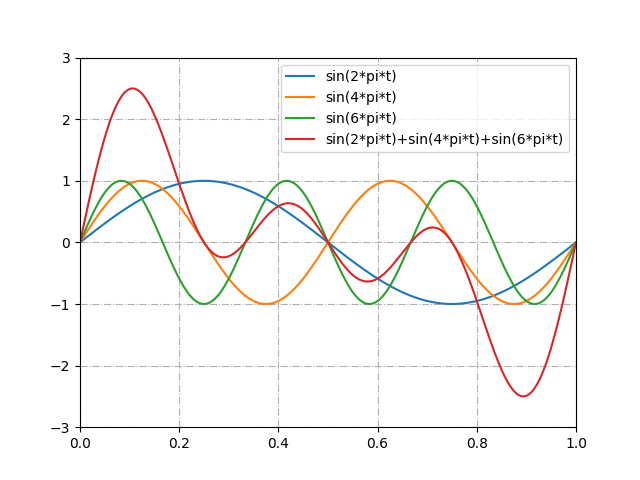
\includegraphics[width=0.4\textwidth]{assets/Figure_1.png}
	\caption{$\sin(2\cdot\pi\cdot t)+\sin(4\cdot\pi\cdot t)+\sin(8\cdot\pi\cdot t)$}
\end{figure}
\begin{enumerate}
	\item 一般表示为:
	      \begin{equation}\label{vtri}
		      f(t)=\sum\limits_{k=1}^n\ A_k\cdot \sin(2\cdot \pi\cdot k\cdot t+\phi_k)
	      \end{equation}

	      这里使用$\cos$也没有关系,但是这节课里就钦定了$\sin$。
	\item 由上图可以看出,整体的函数在周期最长的函数重复的时候才重复,可以说周期最长的函数奠定了整个函数的基调。$k=1​$时,$T=\frac{2\cdot \pi}{2\cdot \pi}=1​$,周期最长,所以$k=1​$的项被称为fundamental wave。而$k>1​$的项被称为harmonic wave。
\end{enumerate}

\section{Fourier Series的两种表达方式}
\subsection{三角函数形式表示}
我们把\eqref{vtri}展开:
\begin{align*}
	      & f(t)                                                                                                   \\
	=     & \sum\limits_{k=1}^n\ A_k\cdot \sin(2\cdot\pi\cdot k\cdot t+\phi_k)                                     \\
	=     & \sum\limits_{k=1}^n\ [A_k\cdot \sin(2\cdot\pi\cdot k\cdot t)                                           \\
	\cdot & \cos(\phi_k)+A_k\cdot \cos(2\cdot \pi\cdot k\cdot t)\cdot \sin(\phi_k)]                                \\
	=     & \sum\limits_{k=1}^n\ [a_k\cdot \sin(2\cdot\pi\cdot k\cdot t) +b_k\cdot \cos(2\cdot \pi\cdot k\cdot t)]
\end{align*}

其中:
$$
	\left\{
	\begin{array}{lr}
		a_k=A_k\cdot \cos(\phi_k) \\
		b_k=A_k\cdot \sin(\phi_k)
	\end{array}
	\right.
$$

所以我们得到:
\begin{equation}\label{vtri2}
	f(t) =\sum\limits_{k=1}^n\ [a_k\cdot \sin(2\cdot\pi\cdot k\cdot t) +b_k\cdot \cos(2\cdot \pi\cdot k\cdot t)]
\end{equation}
\subsection{复指形式表示}
因为根据\eqref{vtri2}的展开,所以我们令(为什么这么令我也不知道,反正老师就是突然跳到这一步。他想怎么干就怎么干吧……):
\begin{equation}
	f(t)=\sum\limits_{k=-n}^n\ c_k\cdot e^{2\cdot \pi \cdot i \cdot k \cdot t}
\end{equation}

\section{Fourier Series的对称性}
\subsection{欧拉公式Euler's Formula}
\begin{equation}
	e^{2\cdot \pi\cdot i\cdot k\cdot t} =  \cos(2\cdot \pi\cdot k\cdot t)+i\cdot \sin(2\cdot \pi\cdot k\cdot t)
\end{equation}
\begin{equation}
	\cos(2\cdot \pi\cdot k\cdot t)=\frac{e^{2\cdot \pi\cdot i\cdot k\cdot t+}+e^{-2\cdot \pi\cdot i\cdot k\cdot t}}{2}
\end{equation}
\begin{equation}
	\sin(2\cdot \pi\cdot k\cdot t)=\frac{e^{2\cdot \pi\cdot i\cdot k\cdot t+}-e^{-2\cdot \pi\cdot i\cdot k\cdot t}}{2\cdot i}
\end{equation}
\subsection{Fourier Series的对称性}
假设​Signal是一个实Signal(real Signal),则Signal中没有虚部,有​$f(t)=\overline {f(t)}$:
\begin{align*}
	  & f(t)                                                                                        \\
	= & \sum\limits_{k=-n}^n\ c_k\cdot e^{2\cdot \pi \cdot i \cdot k \cdot t}                       \\
	= & \overline{\sum\limits_{k=-n}^n\ c_k\cdot e^{2\cdot \pi \cdot i \cdot k \cdot t}}            \\
	= & \sum\limits_{k=-n}^n\ \overline{c_k}\cdot \overline{e^{2\cdot \pi \cdot i \cdot k \cdot t}} \\
	= & \sum\limits_{k=-n}^n\ \overline{c_k}\cdot e^{-2\cdot \pi \cdot i \cdot k \cdot t}
\end{align*}

因为$\sum\limits_{k=-n}^n=\sum\limits_{k=n}^{-n}$,所以把$k$变成$-k$,得:
\begin{align*}
	  & f(t)                                                                        \\
	= & \sum\limits_{k=-n}^n\ c_k\cdot e^{2\cdot \pi \cdot i \cdot k \cdot t}       \\
	= & \sum\limits_{-k=-n}^n\ c_{-k}\cdot e^{2\cdot \pi \cdot i \cdot k \cdot t}   \\
	= & \sum\limits_{k=n}^{-n}\ c_{-k}\cdot e^{-2\cdot \pi \cdot i \cdot k \cdot t} \\
	= & \sum\limits_{k=-n}^n\ c_{-k}\cdot e^{-2\cdot \pi \cdot i \cdot k \cdot t}
\end{align*}

由上面两个推导知:
$$
	f(x)=\sum\limits_{k=-n}^n \overline{c_k}\cdot e^{-2\cdot \pi \cdot i \cdot k \cdot t}=\sum\limits_{k=-n}^n c_{-k}\cdot e^{-2\cdot \pi \cdot i \cdot k \cdot t}
$$


所以得到:
\begin{equation}
	c_{-k}=\overline{c_k}
\end{equation}

那么我们可知:
\begin{align*}
	  & c_k\cdot e^{2\cdot \pi\cdot i\cdot k\cdot t}+c_{-k}\cdot e^{2\cdot \pi\cdot i\cdot (-k)\cdot t}                 \\
	= & c_k\cdot e^{2\cdot \pi\cdot i\cdot k\cdot t}+c_{-k}\cdot e^{-2\cdot \pi\cdot i\cdot k\cdot t}                   \\
	= & c_k\cdot e^{2\cdot \pi\cdot i\cdot k\cdot t}+\overline{c_k}\cdot e^{\overline{2\cdot \pi\cdot i\cdot k\cdot t}} \\
	= & c_k\cdot e^{2\cdot \pi\cdot i\cdot k\cdot t}+\overline{c_k\cdot e^{2\cdot \pi\cdot i\cdot k\cdot t}}            \\
	= & 2\cdot \Re\{C_k\cdot e^{2\cdot \pi \cdot i\cdot k\cdot t}\}
\end{align*}

所以$c_k\cdot e^{2\cdot \pi\cdot i\cdot k\cdot t}+c_{-k}\cdot e^{2\cdot \pi\cdot i\cdot (-k)\cdot t}$为一个实数。$\sum\limits_{k=-n}^n\ c_k\cdot e^{2\cdot \pi \cdot i \cdot k \cdot t}$可以表示一个实数。

\section{从三角函数到复指形}
\subsection{从三角函数到复指形}
\begin{align*}
	  & f(t)                                                                                                                      \\
	= & \sum\limits_{k=1}^n\ [a_k\cdot \sin(2\cdot\pi\cdot k\cdot t)                                                              \\
	+ & b_k\cdot \cos(2\cdot \pi\cdot k\cdot t)]+\frac{A_0}{2}                                                                    \\
	= & \sum\limits_{k=1}^n\ (a_k\cdot \frac{e^{2\cdot \pi\cdot i\cdot k\cdot t}- e^{-2\cdot \pi\cdot i\cdot k\cdot t}}{2\cdot i} \\
	+ & b_k\cdot \frac{e^{2\cdot \pi\cdot i\cdot k\cdot t+}+e^{-2\cdot \pi\cdot i\cdot k\cdot t}}{2})+\frac{A_0}{2}               \\
	= & \sum\limits_{k=1}^n\ (\frac{b_k-i\cdot a_k}{2}\cdot e^{2\cdot \pi\cdot i\cdot k\cdot t}                                   \\
	+ & \frac{b_k+i\cdot a_k}{2}\cdot e^{-2\cdot \pi\cdot i\cdot k\cdot t})+\frac{A_0}{2}
\end{align*}
设$c_0=\frac{1}{2}\cdot A_0$;$c_k=\frac{b_k-i\cdot a_k}{2}$;$c_{-k}=\overline{c_{k}}=\frac{b_k+i\cdot a_k}{2}$则:
\begin{align*}
	  & f(t)                                                                                                                          \\
	= & \sum\limits_{k=1}^n\ (c_k\cdot e^{2\cdot \pi\cdot k\cdot t}+c_{-k}\cdot e^{-2\cdot \pi\cdot k\cdot t})+c_0                    \\
	= & \sum\limits_{k=1}^n\ c_k\cdot e^{2\cdot \pi\cdot k\cdot t}+\sum\limits_{k=1}^n\ c_{-k}\cdot e^{-2\cdot \pi\cdot k\cdot t}+c_0 \\
	= & \sum\limits_{k=1}^n\ c_k\cdot e^{2\cdot \pi\cdot k\cdot t}+\sum\limits_{k=-1}^{-n}\ c_k\cdot e^{2\cdot \pi\cdot k\cdot t}+c_0 \\
	= & \sum\limits_{k=-n\ k\neq0}^n\ c_k\cdot e^{2\cdot \pi\cdot k\cdot t}+c_0
\end{align*}

为了表示一般的周期现象,光求$\sum\limits_{k=-n}^n$是不够的,我们必须考虑对周期Signal进行无限项求和,即求:$\sum\limits_{k=-\infty}^\infty$。

We can use high frequencies to make sharp corners.
There is discontinuity in some high derivative that means that you are gonna have trouble repeating that phenomenon as a finite sum.
You are gonna have to make N layers and layers to represent it more and more accurately.

由于$\cos(x)$和$\sin(x)$是连续且无限可微分的,所以有限的$\cos(x)$或$\sin(x)$之和不能表示离散的函数或者不无限可微分的函数。
%TODO:c_0到底怎么解决???
所以最终:
\begin{equation}
	f(t)=\sum\limits_{k=-\infty}^\infty\ c_k\cdot e^{2\cdot \pi\cdot k\cdot t}+c_0
\end{equation}
\subsection{求解$c_k$}
我们由上面的推导可知:
\begin{align*}
	c_{-k} & =\overline{c_k}        \\
	c_0    & =c_{-0}=\overline{c_0}
\end{align*}

$f(t)=\sum\limits_{k=-\infty}^\infty c_k\cdot e^{2\cdot \pi \cdot i \cdot k \cdot t}$,取出其中任意一项$c_m\cdot e^{2\cdot \pi \cdot i\cdot m\cdot t} \quad m\in[-\infty,\infty]$:
\begin{align*}
	  & c_m                                                                                                                                                                 \\
	= & f(t)-\sum\limits_{k\neq m}^\infty c_k\cdot e^{2\cdot \pi\cdot i\cdot k\cdot t}                                                                                      \\
	= & e^{-2\cdot \pi \cdot i\cdot m\cdot t}\cdot f(t)-\sum\limits_{k\neq m}^\infty c_k\cdot e^{2\cdot \pi\cdot i\cdot m\cdot t}\cdot e^{-2\cdot \pi\cdot i\cdot k\cdot t} \\
	= & e^{-2\cdot \pi\cdot i\cdot m\cdot t}\cdot f(t)-\sum\limits_{k\neq m}^\infty c_k\cdot e^{2\cdot \pi\cdot i\cdot (k-m)\cdot t}
\end{align*}

对等式两边同时积分得到:
$$
	c_m=\int_0^1\ [e^{-2\cdot \pi\cdot i\cdot m\cdot t}\cdot f(t)-\sum\limits_{k\neq m}^\infty\ c_k\cdot e^{2\cdot \pi\cdot i\cdot (k-m)\cdot t}]\ dt
$$

因为$k\neq m$,所以$\int_0^1\ e^{2\cdot \pi\cdot i\cdot (k-m)\cdot t}\ dt=0$(该结论的证明后面有)。所以有:
$$
	c_m=\int_0^1 \ e^{-2\cdot \pi\cdot i\cdot m\cdot t}\cdot f(t)\ dt
$$

\subsection{傅立叶参数 Fourier Coefficient}
我们用新记号$\hat{f}(k)$表示$c_k$:
\begin{equation}
	\hat{f}(k)=\int_0^1 \ e^{-2\cdot \pi\cdot i\cdot m\cdot t}\cdot f(t)\ dt
\end{equation}

因为是Fourier Series的项,所以变量为频率$k$。
Fourier Series用以下方式表示:
\begin{equation}
	f(t)=\sum\limits_{k=-\infty}^\infty\ \hat{f}(k)\cdot e^{2\cdot \pi\cdot i\cdot k\cdot t }
\end{equation}

因为在Time Domain中观察,所以变量为时间变量$t$。
这两个式子的指数中:
\begin{enumerate}
	\item $2\cdot \pi$为函数的周期。这个周期来自最初的三角函数的周期设定;
	\item $k​$为Frequency Domain变量,在分析Time Domain的时候作为常数处理;
	\item $t$为Time Domain变量,在分析Frequency Domain时作为常数处理。
\end{enumerate}
\section{通用性验证}
\subsection{适用范围}
\subsubsection{关于三角函数的讨论}
\begin{enumerate}
	\item 由于三角函数是连续的,因此有限项级数不能表示离散的函数;
	\item 由于三角函数是无限可微分的,因此有限项级数不能表示不无限可微分的函数。
\end{enumerate}


\subsubsection{Dirichlet Condition}
一个周期函数在任意一个周期内:
\begin{enumerate}
	\item 有有限个一类间断点;
	\item 有有限个极大值与极小值;
	\item 其绝对值可积。
\end{enumerate}

则可以表示为Fourier Series。
\subsubsection{有限求和}
We can use high frequencies to make sharp corners. There is a discontinuity in some high derivative that means that you are going to have trouble repeating that phenomenon as a finite sum. You are going to take N layers and layers to try to represent it more and more accurately.
\subsection{收敛性}
为什么要讨论收敛?任何非平滑的Signal都会产生无限多个Fourier Series。如果在有限项后截断来得到函数近似,万一级数不收敛于$f(t)$,情况就很糟糕。
\subsubsection{$L_2$收敛}
一般Signal(也包括上述两种情况)的收敛性在分析的时候,不采用逐点判断收敛性的方法,用均方收敛(convergence in the mean)。

如果$\int_{0}^{1}\ |f(t)|^2\ dt<\infty$,且:$\int_{0}^{1}\ |\sum\limits_{k=-n}^{n}\ \hat{f}(k)\cdot e^{-2\cdot \pi\cdot i\cdot k\cdot t\ dt-f(t)}|^2\rightarrow 0\ if\ n\rightarrow \infty$,则可表示为:
$$
	f\in L_2([0,1])
$$
\subsubsection{收敛结论}
\begin{enumerate}
	\item 如果Signal是平滑连续的(连续可微),在所有的$t$处都会收敛于$f(t)$;
	\item 如果Signal是有跳变的,在跳变点将收敛于跳变点前、后的平均值。
	      \begin{figure}[H]
		      \centering
		      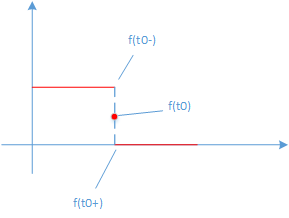
\includegraphics[width=0.4\textwidth]{assets/convergence.png}
		      \caption{跳变函数的收敛性}
	      \end{figure}
\end{enumerate}
\section{函数的内积}
\subsection{函数内积计算方法}
设有复变函数$f,g\in L_2([0,1])$,那么可以把$f,g$分别认为是Vector。求这两个Vector内积的方法为:
\begin{equation}
	(f,g)=\int_0^1\ f(t)\overline{g(t)}\ dt
\end{equation}
\begin{enumerate}
	\item $g(t)​$取共轭函数!!!!!
	\item 当$(f,g)=0$的时候,就可以说$f$与$g​$正交。
\end{enumerate}
\subsection{与Vector类比}
\begin{enumerate}
	\item 类比Vector的模:
	      $$
		      (f,f)=||f||^2=\int_0^1\ |f(t)|^2 \ dt
	      $$
	\item 当$f$与$g​$正交的时候,有函数形式的勾股定理:
	      $$
		      ||f+g||^2=||f||^2+||g||^2
	      $$
\end{enumerate}
\section{Fourier Series与Matrix}
\subsection{空间内的Orthogonal Basis}
空间内一组标准正交Vector:$q_1,q_2,\cdots ,q_n$。空间内任意Vector$\mathbf{v}$有:
\begin{align*}
	v & =x_1\cdot q_1+x_2\cdot q_2+\cdots+x_n\cdot q_n=Q\cdot x \\
	x & =Q^{-1}\cdot v                                          \\
\end{align*}

因为$Q$为正交Matrix,所以$Q^T=Q^{-1}$,所以$x=Q^T\cdot v$。

因为$q_i$为标准Orthogonal Basis,所以$q_i^T\cdot q_j=0$。

所以$x_i=q_i^T\cdot v$。Vector与标准Orthogonal Basis的点乘,求得各分量。
\subsection{Orthogonal Basis}
\subsubsection{三角函数的Orthogonal Basis}
正弦余弦函数一定正交:
$$
	\int_0^{\frac{2\cdot \pi}{n}}\ \cos(n\cdot x)\sin(n\cdot x)=0
$$

相同频率的正弦函数不正交:
$$
	\int_0^{\frac{2\cdot \pi}{n}}\ \sin(n\cdot x)\sin(n\cdot x)=1
$$

相同频率的余弦函数不正交:
$$
	\int_0^{\frac{2\cdot \pi}{n}}\ \cos(n\cdot x)\cos(n\cdot x)=1
$$

由此性质,我们可以将$\sin(2\cdot \pi\cdot m \cdot t)$和$\cos(2\cdot \pi\cdot m \cdot t)$看作Fourier Series上的Orthogonal Basis,來求解Fourier Coefficient。
\subsubsection{复指函数的Orthogonal Basis}
\begin{align*}
	  & (e^{2\cdot \pi\cdot i\cdot m\cdot t},e^{2\cdot \pi\cdot i\cdot n\cdot t})                      \\
	= & \int_0^1 \ e^{2\cdot \pi\cdot i\cdot m\cdot t}\cdot e^{2\cdot \pi\cdot i\cdot (-n)\cdot t}\ dt \\
	= & \int_0^1 \ e^{e^{2\cdot \pi\cdot i\cdot (m-n)\cdot t}}\ dt                                     \\
	= & \rsx{\frac{e^{2\cdot \pi\cdot i\cdot (m-n)\cdot t}}{2\cdot \pi \cdot i \cdot(m-n)}}_0^1
\end{align*}

展开$e^{2\cdot \pi\cdot i\cdot (m-n)\cdot t}$:
\begin{align*}
	  & e^{2\cdot \pi\cdot i\cdot (m-n)\cdot t}                                       \\
	= & \cos(2\cdot \pi \cdot t\cdot(m-n))+i \cdot \sin(2\cdot \pi \cdot t\cdot(m-n))
\end{align*}

因为$m,n\in \mathbb{Z}$,所以$m-n\in \mathbb{Z}$;所以$\cos(2\cdot \pi \cdot t\cdot(m-n))=1$;所以$\sin(2\cdot \pi \cdot t\cdot(m-n))=0$;所以$e^{2\cdot \pi\cdot i\cdot (m-n)\cdot t}-e^0=0$。

因此$e^{2\cdot \pi i\cdot k \cdot t}$被称为Fourier Transform中的Orthogonal Basis。
$$
	\begin{cases}
		(e^{2\cdot \pi\cdot i\cdot m\cdot t},e^{2\cdot \pi\cdot i\cdot m\cdot t}) & =1 \\
		(e^{2\cdot \pi\cdot i\cdot m\cdot t},e^{2\cdot \pi\cdot i\cdot n\cdot t}) & =0
	\end{cases}
$$
\subsection{求解Fourier Coefficient}
\subsubsection{三角函数形}
$f(t)$的三角函数表达式如下:

$$f(t)=\sum\limits_{k=1}^n\ [a_k\cdot \sin(2\cdot\pi\cdot k\cdot t) +b_k\cdot \cos(2\cdot \pi\cdot k\cdot t)]$$

将$f(t)$分别与$\sin(2\cdot \pi\cdot m \cdot t)$和$\cos(2\cdot \pi\cdot m \cdot t)$做内积,可以得到$a_m$和$b_m$:
\begin{align*}
	  & \int_0^1\ f(x)\cdot \sin(2\cdot \pi\cdot m \cdot t)\ dt            \\
	= & \int_0^1\ a_m\cdot \sin^2(2\cdot \pi\cdot m \cdot t)\ dt           \\
	= & \int_0^1\ a_m\cdot \frac{1-\cos(4\cdot \pi\cdot m \cdot t)}{2}\ dt \\
	= & \frac{a_m}{2}                                                      \\
\end{align*}
因此:
$$
	a_m=\frac{\int_0^1\ f(x)\cdot \sin(2\cdot \pi\cdot m \cdot t)\ dt}{\frac{1}{2}}
$$
同理:
$$
	b_m=\frac{\int_0^1\ f(x)\cdot \cos(2\cdot \pi\cdot m \cdot t)\ dt}{\frac{1}{2}}
$$
我们再来看看$c_m$:
\begin{align*}
	  & c_m                                                           \\
	= & \int_0^1 \ e^{-2\cdot \pi\cdot i\cdot m\cdot t}\cdot f(t)\ dt \\
	= & \int_0^1 \ [\cos(-2\cdot \pi\cdot i\cdot m\cdot t)            \\
	+ & i\cdot \sin(-2\cdot \pi\cdot i\cdot m\cdot t)\cdot f(t)]\ dt  \\
	= & \int_0^1 \ [\cos(2\cdot \pi\cdot i\cdot m\cdot t)             \\
	- & i\cdot \sin(2\cdot \pi\cdot i\cdot m\cdot t)\cdot f(t)]\ dt   \\
	= & \frac{b_m-i\cdot a_m}{2}
\end{align*}
与前面得到的结论一致。
\subsubsection{复指函数形}
如果$\mathbf{v}$是单位Vector,那么$(\mathbf{u},\mathbf{v})$是$\mathbf{u}$在$\mathbf{v}$上的投影。

类比到Fourier Series:
\begin{align*}
	  & \hat{f}(k)                                                    \\                                          \\
	= & \int_0^1 \ f(t)\cdot e^{-2\cdot \pi\cdot i\cdot k\cdot t}\ dt \\
	= & (f(t),e^{2\cdot \pi\cdot i\cdot k\cdot t})
\end{align*}

因此Fourier Coefficient\ $\hat{f}(k)$是原函数$f(t)$在$e^{-2\cdot \pi\cdot i\cdot k\cdot t}$上的投影。

几何上的分量:
$$
	\mathbf{a}_{\mathbf{v}}=(\mathbf{a},\mathbf{v})\cdot \mathbf{v}
$$
\begin{enumerate}
	\item 先通过内积得到投影;
	\item 然后用投影乘上代表Vector方向的Orthogonal Basis得到该方向上的分量。
\end{enumerate}

类比到Fourier Series:
\begin{align*}
	  & f(t)                                                                                                             \\
	= & \sum\limits_{k=-\infty}^\infty \ \hat{f}(t)\cdot e^{2\cdot \pi\cdot i\cdot k\cdot t}                             \\
	= & \sum\limits_{k=-\infty}^\infty\ (f,e^{2\cdot \pi\cdot i\cdot k\cdot t})\cdot e^{2\cdot \pi\cdot i\cdot k\cdot t}
\end{align*}

\begin{enumerate}
	\item 函数进行Fourier Series后的每一项,都是函数在不同的Orthogonal Basis$e^{2\cdot \pi\cdot i\cdot k\cdot t}$上的分量。
	\item 反过来,这些分量相加构成完整的原始函数。
\end{enumerate}

下面补充Rayleigh's Identity。几何上,因为$\mathbf{c}^2=\mathbf{a}^2+\mathbf{b}^2$,所以$(\mathbf{a},\mathbf{b})=0$。类比到Fourier Series,帕塞瓦尔定理的定义如下:
$$
	\int_0^1\ |f(t)|^2\ dt=\sum\limits_{k=-\infty}^{\infty}\ |\hat{f}(x)|^2
$$

Fourier Transform后的项互为正交项,正交项内积为$0$。
\section{Convolution}
It is convolution in time, multiplication in frequency.

一般来说,Frequency Domain的运算会比Time Domain简单许多,因为Frequency Domain只需执行相乘运算。
\subsection{定义}
设$f(t)$、$g(t)$是$\mathbb{R}$上两个可积函数,作积分:
$$
	\int_{-\infty}^\infty\ f(\tau)\cdot g(t-\tau)\ d\tau
$$
可以证明,关于几乎所有的 $x\in (-\infty ,\infty )$,上述积分是存在的。这样,随着$x$的不同取值,这个积分就定义了一个新函数$h(x)$,称为函数$f$与$g$的Convolution,记为:
$$
	h(x)=(f*g)(t)=\int_{-\infty}^{\infty}\ f(r)\cdot g(t-r)\ dr
$$
\subsection{Convolution与偏微分方程}
偏微分方程的解经常以Convolution的形式出现。Convolution的一方是特解,另一方是给定的初始数据下的初始条件。
\subsection{图解Convolution}
\begin{figure}[H]
	\centering
	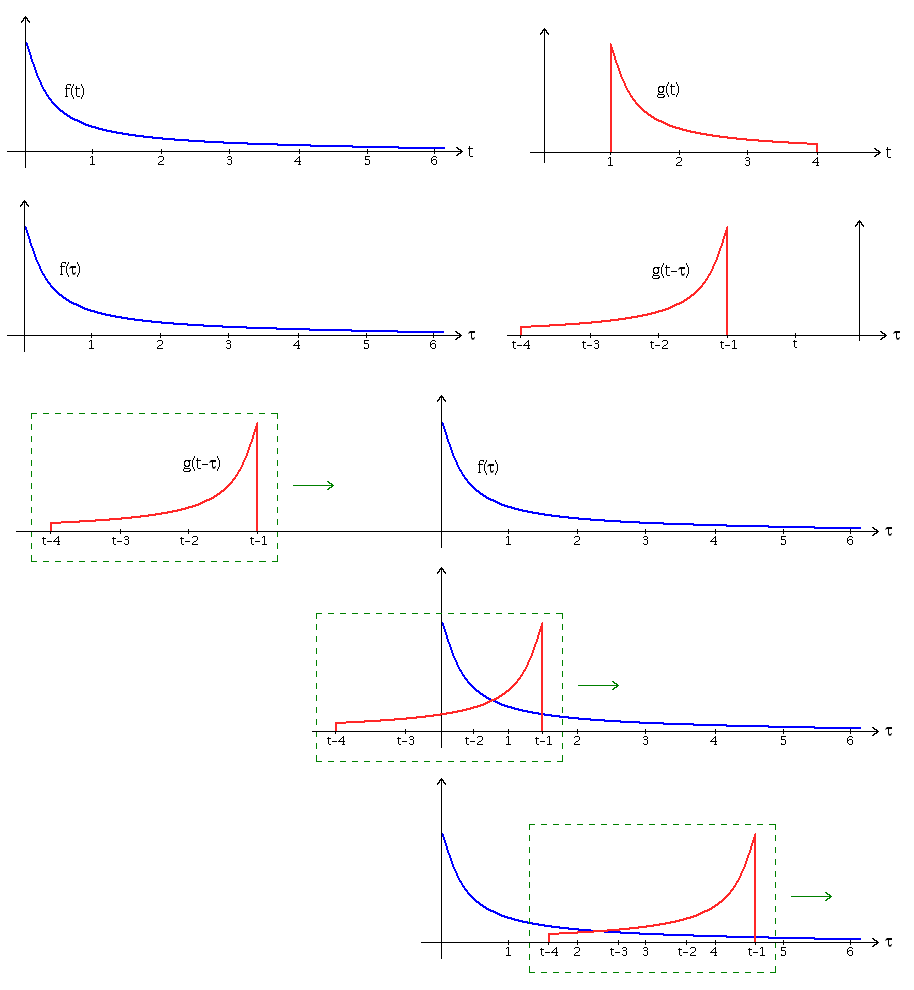
\includegraphics[width=0.4\textwidth]{assets/Convolution.png}
	\caption{图解Convolution}
\end{figure}

\begin{enumerate}
	\item 已知两函数$f(t)$和$g(t)$。上图第一行分别为$f(t)$和$g(t)$。
	\item 首先将两个函数都用$\tau$来表示,从而得到$f(\tau)$和$g(\tau)$。将函数$g(\tau)$向右移动t个单位,得到函数$g(\tau-t)$的图像。将$g(\tau-t)$翻转至纵轴另一侧,得到$g(t-\tau)$的图像。上图第二行两图分别为$f(\tau)$和$g(t-\tau)$。
	\item 由于$\tau$是时间变量,当时间变量(以下简称“时移”)取不同值时,$g(t-\tau)$能沿着$\tau$轴“滑动”。右图第三四五行可理解为“滑动”。
	\item 让$\tau$从$-∞$滑动到$+∞$。两函数交会时,计算交会范围中两函数乘积的积分值。换句话说,我们是在计算一个滑动的的加权总和。也就是使用$g(t-\tau )$当做加权函数,来对$f(\tau)$取加权值。
	\item 最后得到的波形(未包含在此图中)就是$f$和$g$的Convolution。如果$f(t)$是一个单位脉冲,我们得到的乘积就是$g(t)$本身,称为冲激响应。
\end{enumerate}

\end{document}